\section{Deflection Plates}

In order to redirect the beam down the column, in conjunction with the accelerator alignment mechanisms, custom large area deflector plates were employed.
Four plates are arranged on a hollow tube with a square profile, one on each side.
One of each pair is held at ground while the other has a variable potential.
By varying each potential the beam may be turned in flight.

\begin{figure}
  \centering
  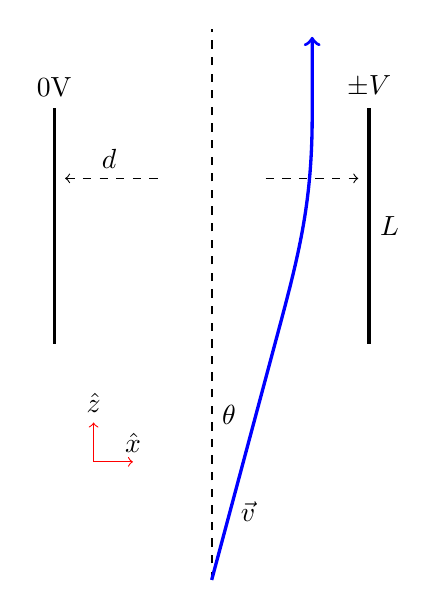
\begin{tikzpicture}
  \draw [very thick]
    (0,0) -- ++(0,3)
      node (left plate) [pos=0.7] {}
      node [above, pos=1] {0V}
  ;
  \draw [very thick]
    (4,0) -- ++(0,3)
      node [right, pos=0.5] {$L$}
      node (right plate) [pos=0.7] {}
      node [above, pos=1] {$\pm V$}
  ;
  \draw [dashed, <->]
    (left plate) -- (right plate)
    node [above, pos=0.15] {$d$}
    node [fill=white, pos=0.5] {\hphantom{XXXX}}
  ;

  \draw [thick, dashed]
    (2,-3) coordinate (start)
      -- ++(0,7)
      node [pos=0.3, right] {$\theta$}
  ;
  \draw [very thick, blue, -> ]
    (start) 
      -- ++(75:3)
        node [right, pos=0.3, black] {$\vec{v}$}
      to [out=75,in=270] ++(0.5,3)
      -- ++(0,1)
  ;

  % axes
  \draw [red, ->] 
    (0.5,-1.5) coordinate (axes start)
    -- ++(0,0.5)
      node [pos=1, above, black] {$\hat{z}$}
  ;
  \draw [red, ->] 
    (axes start) -- ++(0.5,0)
      node [pos=1, above, black] {$\hat{x}$}
  ;
\end{tikzpicture}

  \caption[Schematic diagram of one pair of deflection plates]{
    Schematic diagram of one pair of deflection plates.
    The blue ray represents the path of the pulse as a whole (not to be confused with the plot of a lens).
  }
  \label{fig:deflector_schematic}
\end{figure}

A schematic description of such a system is shown in \ref{fig:deflector_schematic}.
To estimate the required voltage on the plates $V$, consider the applied impulse provided to the beam by the plate's electric field
\begin{gather}
  F \Delta t = m \Delta v \\
  \frac{ e V }{ d } \frac{ L }{ v_z } = m_e \Delta v_x
\end{gather}
where (as seen in the figure) $L$ is the length of the plate (in the direction of travel $\hat{z}$) and $d$ is the separation of the plates.
Then in the small angle approximation, the angle that the plate may correct for is approximately
\begin{equation}
  \theta = \frac{ \Delta v_x }{ v_z } = \frac{ e }{ m_e } \frac{ L }{ d } \frac{ V }{ v_z^2 }
\end{equation}
Using this result, when $L \sim d$ and $v_z = c/3$ a voltage of 1kV will deflect the beam approximately one degree.
These plates therefore are used as a fine adjustment, as opposed to the coarse adjustment provided by aligning the acceleration gap.

\begin{figure}
  \centering
  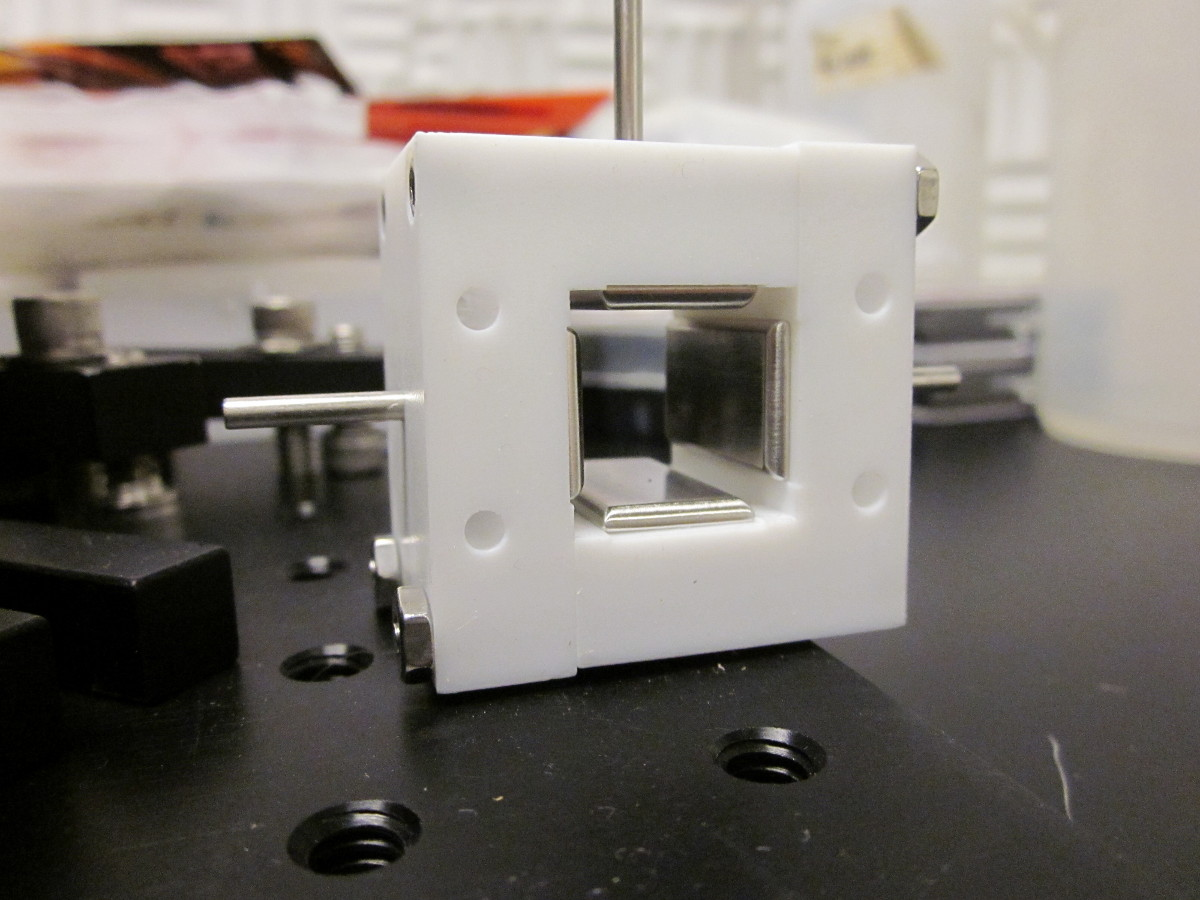
\includegraphics{deflector_plates.jpg}
  \caption[Picture of custom deflector plates]{
    Picture of the custom built deflector plates for use in the UEM at UIC.
    A pair of vertical and horizontal plates are mounted in a non-conductive housing.
    Each plate has a pin for connecting to voltage or ground.
    Clearance drilled holes allow mounting onto the ``eV parts'' cage inside the chamber.
  }
  \label{fig:deflector-plates-pic}
\end{figure}
